\begin{frame}{Sistema solare}
\begin{columns}\begin{column}{0.5\textwidth}
\begin{block}{Radio-datazione meteoriti}

\end{block}
\end{column}\begin{column}{0.5\textwidth}
\begin{block}{Et\'a del Sole}

\end{block}
\end{column}\end{columns}

\end{itemize}
\end{frame}

\begin{wordonframe}{Schema rozzo vincoli ai modelli di formazione}
Caratteristiche pianeti sistema solare
composizione pianeti giganti
MMSN
Si ipotizza che la migrazione causata da interazioni pianeti giganti con gas del disco e poi planetesimi si cruciale per spiegare la configurazione orbitale attuale
condizioni iniziali per formazione planetaria
\end{wordonframe}

\begin{frame}{Sistema Solare e scenario core accretion}
\begin{columns}[T]
	\begin{column}{0.45\textwidth}
	\begin{itemize}
			\item Arricchimento metalli
			\item Oggetti pi\'u antichi hanno et\'a del Sole %($\Omega\tau_{cool}\gg1$): 
			\item numerosa popolazione corpi minori
		\end{itemize}
	\end{column}
	\begin{column}{0.54\textwidth}
		\begin{table}[!ht]
			\begin{flushleft}
\begin{minipage}{.25\linewidth}
	\begin{tabular}{@{}|ccc|@{}}
		\hline
		&\parbox{1.5cm}{Jupiter $317.8\mearth{}$}&\parbox{1.5cm}{Saturn $95.1\mearth{}$}\\
		$M_c$&$0-11\mearth{}$&$9-22\mearth{}$\\
		\hline
		$M_Z$&$1-39\mearth{}$&$1-8\mearth{}$\\
		\hline
		$M_Z^{tot}$&$8-39\mearth{}$&$13-28\mearth{}$\\
		\hline
		$Z/Z_{\odot}$&$1-6$&$6-14$\\
		\hline
	\end{tabular}
\end{minipage}%

\vspace{3mm}
			
			\begin{minipage}{.25\linewidth}
				\centering
				\begin{tabular}{@{}|ccc|@{}}
					\hline
					&\parbox{1.5cm}{Uranus $14.5\mearth{}$}&\parbox{1.5cm}{Neptune $17.1\mearth{}$}\\
					\hline
					$M_{rock}$&$3.7\mearth{}$&$4.2\mearth{}$\\
					\hline
					$M_{ice}$&$9.3\mearth{}$&$10.7\mearth{}$\\
					\hline
					$M_{H/He}$&$1.5\mearth{}$&$2.2\mearth{}$\\
					\hline
				\end{tabular}
			\end{minipage}
					\end{flushleft}
			\caption{Da \cite{baraffe2009physical}.}\label{tab:JSUNcomp}
		\end{table}
	\end{column}
\end{columns}
\end{frame}

\begin{wordonframe}{''ruoli sistema solare'' e intro CA}
[Il sistema solare per primo \'e stato il banco di prova delle teorie di formazione di sistemi planetari: loscenario di core accretion trova giustificazione in alcune caratteristiche del sistema solare e da quest'ultimo \'e possibile stimare in maniera quantitativa la massa del disco protoplanetario da cui ha avuto origine]

I meteoriti pi\'u antichi hanno et\'a compatibile con et\'a del sole quindi \'e plausibile che si siano formati per primi e nello scenario CA trovano collocazione naturale il resto dei corpi minori.
La composizione di giove, saturno e dei pianeti ghiacciati mostra un sostanzioso arricchimento di metalli rispetto al sole: questo sarebbe ovvia conseguenza dell'accrescimento di gas su core solido.

\end{wordonframe}

\begin{frame}{Minimum mass solar nebula}
\begin{columns}[T]
	\begin{column}{0.45\textwidth}
\begin{itemize}
	\item Massa prevista nei modelli GI due ordini di grandezza superiore a MMSN ($Q\gg1$)
\end{itemize}
	\end{column}
	\begin{column}{0.54\textwidth}
			\begin{figure}[!ht]
			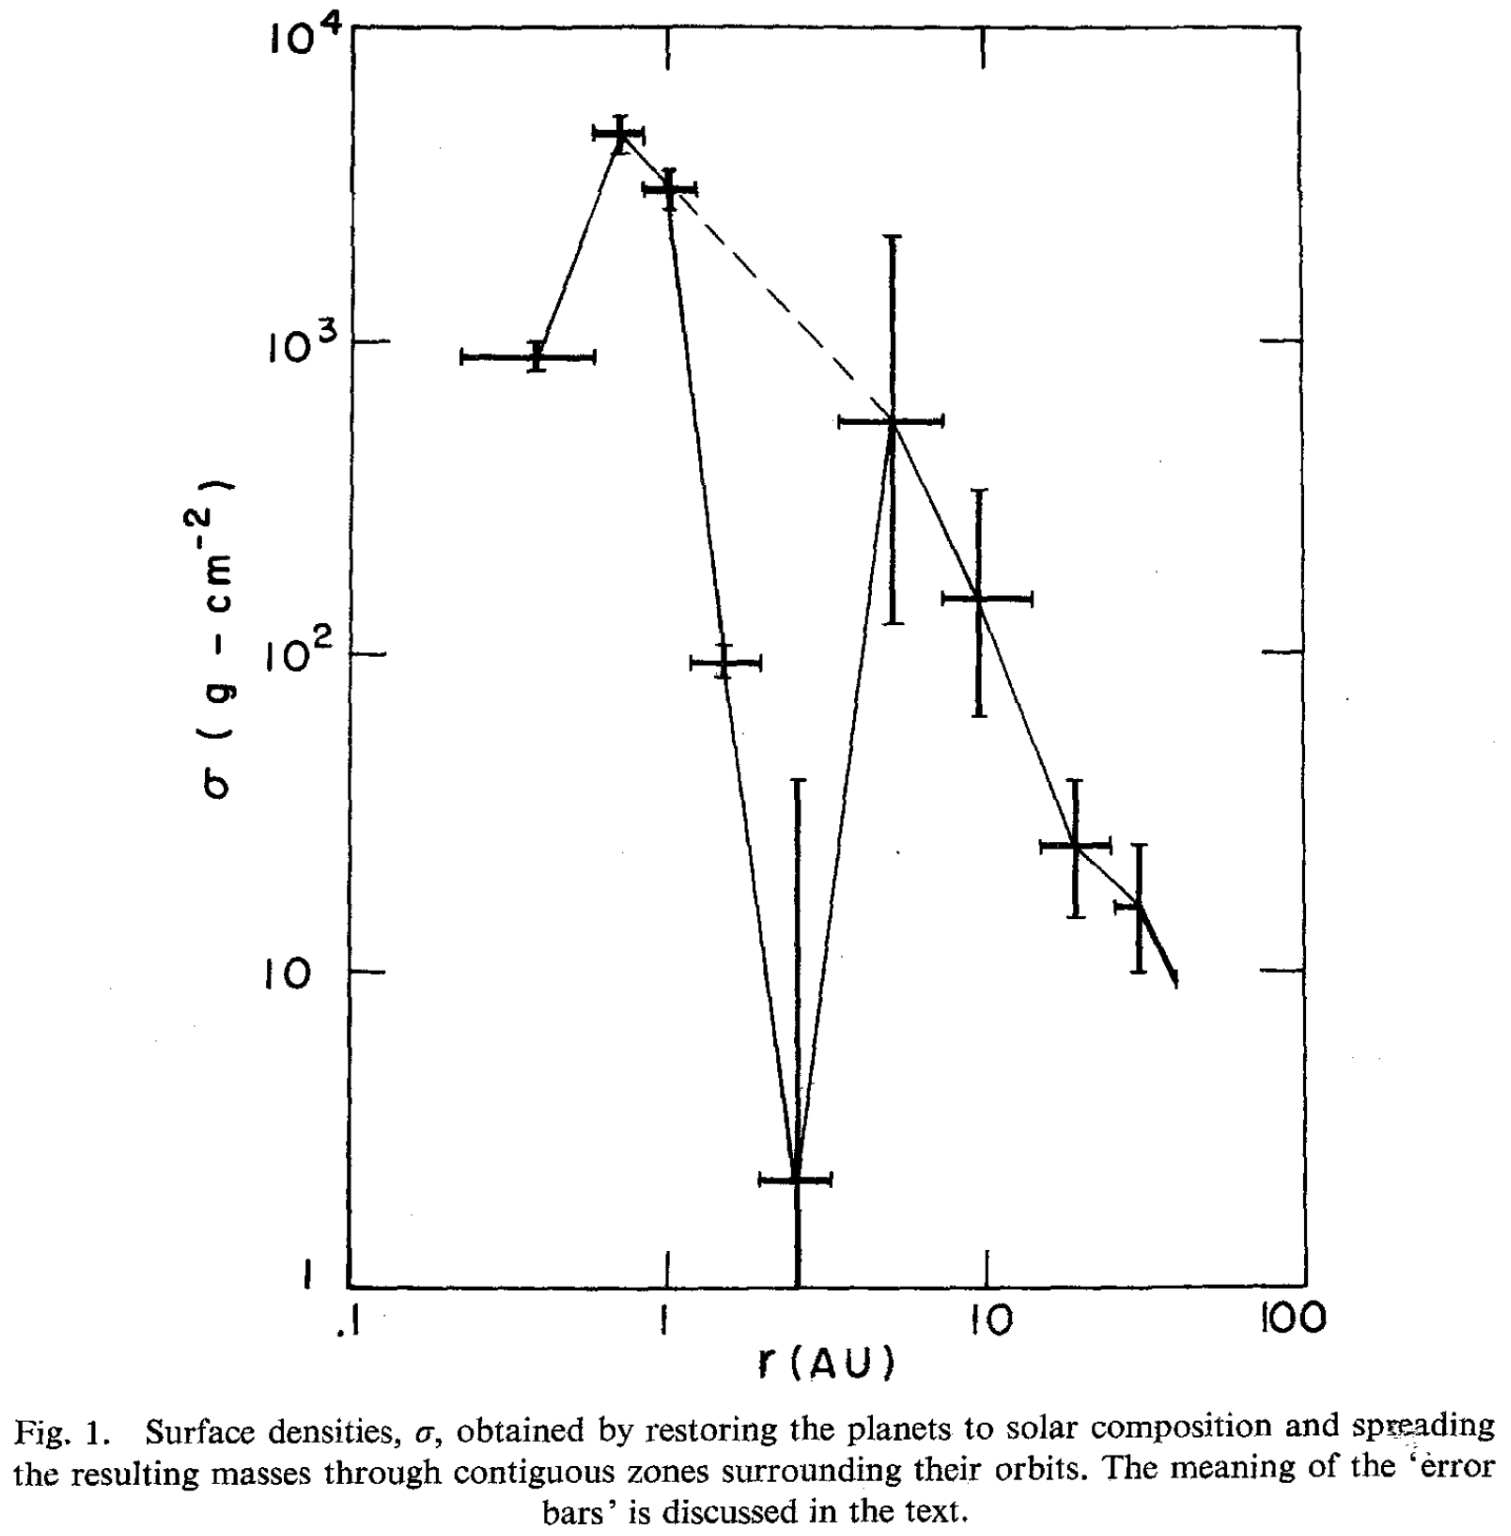
\includegraphics[trim={0cm 5cm 0 0cm},clip, width=0.99\textwidth]{Snebuladensity}
			\caption{Da \cite{weidenschilling1977distribution}.}\label{fig:Snebuladensity}
		\end{figure}
	\end{column}
\end{columns}
\end{frame}

\begin{wordonframe}{Core accretion e MMSN}

Inoltre \'e possibile determinare dalla configurazione attuale,aggiungendo la massa di H/He per ripristinare composizione solare, una stima inferiore della massa iniziale 
\begin{align*}
&\Sigma\propto r\expy{-3/2}
&M\approx0.02\msun{}
\end{align*}

\end{wordonframe}
